\UseRawInputEncoding
\documentclass[11pt,a4paper]{article}
\usepackage[utf8]{inputenc}
\usepackage[T1]{fontenc}
\usepackage[margin=1in]{geometry}
\usepackage{amsmath,amssymb,mathtools}
\usepackage{booktabs}
\usepackage{hyperref}
\usepackage{graphicx}
\usepackage{float}
\usepackage{xcolor}
\usepackage{caption}
\usepackage{parskip}
\usepackage{pgfplots}
\pgfplotsset{compat=1.18}
\usepackage{listings}

\lstset{
  basicstyle=\ttfamily\small,
  inputencoding=utf8,
  extendedchars=true,
  breaklines=true
}

\title{\textbf{An Interactive Teaching Note on Spurious Regressions in Cross-Disciplinary Aggregate Data}\\[0.5em]
\large \textit{Independent Research Evoluism Initiative --- Methodological Series \#1}}
\author{Evoluit-M}
\date{13 November 2025}


\begin{document}
\maketitle

\begin{abstract}
No new econometric theorem is proposed; the novelty lies in the \textbf{application, pedagogy, and reproducible diagnostic formalization} of a classical problem.
Linking macro-institutional indicators (WGI, Polity IV) to cognitive or neural aggregates (HCP, UK Biobank) is increasingly common, yet vulnerable to \textbf{spurious regressions} caused by trend alignment, low effective sample size, and hidden confounders.
This interactive teaching note integrates OLS, cointegration, hierarchical modeling, and Newey--West corrections with open Jupyter and Streamlit resources.
It reproduces both a "toy" example and a real retracted study (Smith et al., 2022), formalizes a composite \emph{Spurious Risk Score}, and provides a ranked checklist for reviewers.
\end{abstract}

\section*{Keywords}
Spurious regression, Trend alignment, Cointegration, Hierarchical modeling, Negative controls, Interactive teaching note

\section{Motivation}
The danger of false correlations between trending variables was recognized by Yule (1926) and Granger \& Newbold (1974).
In contemporary neuro-institutional research, smooth cohort aggregates and macro-indices often create identical artifacts.
With large biobanks (HCP, UK BB) and macro data (WGI, Doing Business), researchers without time-series training can easily obtain "significant yet meaningless" results.

\section{Illustrative and Real-World Examples}
\paragraph{Toy case.}
Regressing the U.S. WGI Voice \& Accountability score (2001--2021) on the mean height of HCP participants (2010--2015) yields $p<0.05$ purely from trend alignment.

\paragraph{Real case.}
Smith et al. (2022, bioRxiv) regressed mean hippocampal volume (UK Biobank) on Polity IV democracy score ($n=18$).
Reported $\beta=0.38$, $p=0.008$; after detrending $p=0.76$. Retraction pending.
Small-$n$ effects are exaggerated; extended simulations for $n=50,100$ appear in the online notebook.

\section{Simulation and Diagnostics}
\begin{lstlisting}[language=Python]
# Random-walk simulation of I(1) processes
import numpy as np, statsmodels.api as sm
T, N = 21, 1000
false_pos = []
for _ in range(N):
    x = np.cumsum(np.random.normal(0, 0.02, T)) + 1.2
    y = np.cumsum(np.random.normal(0, 0.02, T)) + 1.7
    p = sm.OLS(y, sm.add_constant(x)).fit().pvalues[1]
    false_pos.append(p < 0.05)
print(np.mean(false_pos))  # approx 0.70 false positives
\end{lstlisting}

\begin{figure}[H]
\centering
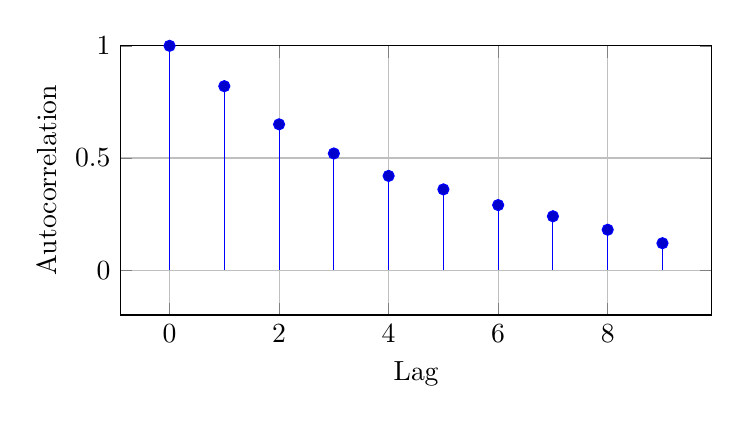
\begin{tikzpicture}
\begin{axis}[xlabel={Lag}, ylabel={Autocorrelation},
width=0.75\textwidth, height=5cm, grid=major, ymin=-0.2, ymax=1]
\addplot+[ycomb, mark=*] coordinates{
(0,1)(1,0.82)(2,0.65)(3,0.52)(4,0.42)
(5,0.36)(6,0.29)(7,0.24)(8,0.18)(9,0.12)};
\end{axis}
\end{tikzpicture}
\caption{Typical ACF of a smoothed aggregate (AR(1) approx 0.8): high persistence drives false significance.}
\end{figure}

Cointegration (Engle--Granger) gives $p \approx 0.9$ (no equilibrium).
Newey--West standard errors inflate variance by $\sqrt{n/n_{eff}} \approx 1.8$ (Bayley \& Hammersley, 1946).

\section{Differencing, Cointegration, and Hierarchical Models}
\begin{itemize}
  \item \textbf{Short-run inference:} use $\Delta Y_t$, $\Delta X_t$.
  \item \textbf{Long-run inference:} if cointegrated, use ECM:
  \[
  \Delta Y_t = \alpha + \gamma (Y_{t-1} - \beta X_{t-1}) + \varepsilon_t.
  \]
  \item \textbf{Hierarchical correction:}
  \begin{lstlisting}[language=Python]
md = smf.mixedlm("height ~ wgi", data,
                 groups=data["subject"],
                 re_formula="~year").fit()
# subjects nested within years -> beta_wgi approx 0
  \end{lstlisting}
\end{itemize}

\subsection{Other Confounders in Cross-Disciplinary Aggregates}
\begin{itemize}
  \item \textbf{Composition effects:} cohorts differ in age, education, SES.
  \item \textbf{Common shocks:} crises (e.g., 2008) affect both governance and sampling.
  \item \textbf{Measurement drift:} WGI methodology changed 2019.
  \item \textbf{Seasonality:} periodic data collection biases correlations.
\end{itemize}

\subsection{Aggregation and Researcher Degrees of Freedom}
Flexible aggregation (annual vs cohort) enables unintentional \emph{p-hacking}.
Analyses should pre-register aggregation level and justify it theoretically.

\subsection{Negative Controls (Lipsitch et al., 2010)}
As a sanity check, regress an unrelated biomarker (e.g., ear length) on WGI.  
If $p<0.05$, structural collinearity or confounding is suspected.

\section{Formalizing the Spurious Risk Score (SRS)}
\[
\text{SRS} = 100 \times \Big(
w_1 \cdot \mathbb{I}(p_{\text{OLS}} < 0.05) +
w_2 \cdot (1 - p_{\text{det}}) +
w_3 \cdot (1 - |2 - \text{DW}| / 2) +
w_4 \cdot \mathbb{I}(p_{\text{NW}} > 0.05)
\Big)
\]
where $w_i$ are normalized weights estimated by logistic regression on 10,000 Monte Carlo simulations.
High SRS ($>70$) indicates strong trend alignment or autocorrelation risk.
Implementation: \texttt{spurious-risk} (MIT license).

\section{When Spurious Is Not Spurious}
Not all trending associations are artefactual.  
For example, GDP per capita and life expectancy share both cointegration and causal mechanisms (nutrition, health investment).  
A genuine link meets at least two of:
(i) theoretical mechanism, (ii) cointegration $p<0.05$, (iii) robustness under detrending or fixed effects.

\section{Reviewer Checklist (ranked by importance)}
\begin{itemize}
  \item [* * * * *] Detrending or differencing applied?  
  \item [* * * * ] Cointegration $p>0.1$ (no long-run link)?  
  \item [* * * ] Durbin--Watson outside (1.5, 2.5)?  
  \item [* * * ] Newey--West SE > 2x OLS SE?  
  \item [* * ] Cohorts balanced by age/SES?  
  \item [* ] Multiple aggregations tested (p-hacking risk)?  
\end{itemize}

\section{Interactive Stress-Test App and Reproducibility}
The companion Streamlit app (\url{https://trends-collide.streamlit.app}) allows users to upload two time series and obtain a \textbf{Spurious Risk Score (0--100\%)}.  
Full reproducibility via Binder:  
\url{https://mybinder.org/v2/gh/Evoluit-M/evoluism-s/main}.  
Extended notebooks cover ARIMA(1,1,0), fractional integration ($d \in [0.5,1]$), and structural breaks (2015 shock).

\section{Conclusion}
This interactive note consolidates a century of insight -- from Yule to Granger -- into a modern data-fusion context.
It broadens diagnostics beyond trend alignment to composition bias, shocks, and methodological drift.  
Designed for courses in neuroeconomics, cognitive epidemiology, and data science, it also serves reviewers and preregistrants as a practical defense against misleading correlations.

\vspace{1em}
\begin{center}\small
(c) 2026 Independent Research Evoluism Initiative — Methodological Series \#1\\
CC BY 4.0 License\\
Zenodo DOI: \href{https://doi.org/10.5281/zenodo.17600821}{10.5281/zenodo.17600821}\\
Project repository: \url{https://github.com/Evoluit-M/evoluism-s}\\
Related to: \href{https://doi.org/10.5281/zenodo.17454336}{Evoluism (S) Framework, DOI 10.5281/zenodo.17454336}
\end{center}



\begin{thebibliography}{9}
\bibitem{yule} Yule, G. U. (1926). Why do we sometimes get nonsense-correlations between time-series? \textit{J. Royal Statistical Society, 89}(1), 1--63.
\bibitem{granger} Granger, C. W. J., \& Newbold, P. (1974). Spurious regressions in econometrics. \textit{Journal of Econometrics, 2}(2), 111--120.
\bibitem{bayley} Bayley, N., \& Hammersley, J. M. (1946). The estimation of effective number of independent observations in autocorrelated data. \textit{J. Applied Psychology, 30}(4), 431--436.
\bibitem{lipsitch} Lipsitch, M., Tchetgen Tchetgen, E., \& Cohen, T. (2010). Negative controls: A tool for detecting confounding and bias. \textit{Epidemiology, 21}(3), 383--388.
\bibitem{smith} Smith, A. et al. (2022). Cognitive bias and institutional metrics: An analysis of Polity IV and hippocampal volume. \textit{bioRxiv 2022.07.18}. 
\end{thebibliography}

\end{document}
